%%%%%%%%%%%%%%%%%%%%%%%%%%%%%%%%%%%%%%%%%
% Arsclassica Article
% LaTeX Template
% Version 1.1 (10/6/14)
%
% This template has been downloaded from:
% http://www.LaTeXTemplates.com
%
% Original author:
% Lorenzo Pantieri (http://www.lorenzopantieri.net) with extensive modifications by:
% Vel (vel@latextemplates.com)
%
% License:
% CC BY-NC-SA 3.0 (http://creativecommons.org/licenses/by-nc-sa/3.0/)
%
%%%%%%%%%%%%%%%%%%%%%%%%%%%%%%%%%%%%%%%%%

%----------------------------------------------------------------------------------------
%	PACKAGES AND OTHER DOCUMENT CONFIGURATIONS
%----------------------------------------------------------------------------------------

\documentclass[
10pt, % Main document font size
a4paper, % Paper type, use 'letterpaper' for US Letter paper
oneside, % One page layout (no page indentation)
%twoside, % Two page layout (page indentation for binding and different headers)
headinclude,footinclude, % Extra spacing for the header and footer
BCOR5mm, % Binding correction
]{scrartcl}

%%%%%%%%%%%%%%%%%%%%%%%%%%%%%%%%%%%%%%%%%
% Arsclassica Article
% Structure Specification File
%
% This file has been downloaded from:
% http://www.LaTeXTemplates.com
%
% Original author:
% Lorenzo Pantieri (http://www.lorenzopantieri.net) with extensive modifications by:
% Vel (vel@latextemplates.com)
%
% License:
% CC BY-NC-SA 3.0 (http://creativecommons.org/licenses/by-nc-sa/3.0/)
%
%%%%%%%%%%%%%%%%%%%%%%%%%%%%%%%%%%%%%%%%%

%----------------------------------------------------------------------------------------
%	REQUIRED PACKAGES
%----------------------------------------------------------------------------------------

\usepackage[
nochapters, % Turn off chapters since this is an article
beramono, % Use the Bera Mono font for monospaced text (\texttt)
eulermath,% Use the Euler font for mathematics
pdfspacing, % Makes use of pdftex’ letter spacing capabilities via the microtype package
dottedtoc % Dotted lines leading to the page numbers in the table of contents
]{classicthesis} % The layout is based on the Classic Thesis style

\usepackage{arsclassica} % Modifies the Classic Thesis package

\usepackage[T1]{fontenc} % Use 8-bit encoding that has 256 glyphs

\usepackage[utf8]{inputenc} % Required for including letters with accents

\usepackage{graphicx} % Required for including images
\graphicspath{{figures/eps/}} % Set the default folder for images

\usepackage{enumitem} % Required for manipulating the whitespace between and within lists

\usepackage{lipsum} % Used for inserting dummy 'Lorem ipsum' text into the template

\usepackage{subfig} % Required for creating figures with multiple parts (subfigures)

\usepackage{amsmath,amssymb,amsthm} % For including math equations, theorems, symbols, etc

\usepackage{varioref} % More descriptive referencing

\usepackage{listings}

\usepackage{etoolbox}

% work-around for bug not showing section numbers
\makeatletter
\patchcmd{\ttlh@hang}{\parindent\z@}{\parindent\z@\leavevmode}{}{}
\patchcmd{\ttlh@hang}{\noindent}{}{}{}
\makeatother
% end work-around

%----------------------------------------------------------------------------------------
%	THEOREM STYLES
%---------------------------------------------------------------------------------------

\theoremstyle{definition} % Define theorem styles here based on the definition style (used for definitions and examples)
\newtheorem{definition}{Definition}

\theoremstyle{plain} % Define theorem styles here based on the plain style (used for theorems, lemmas, propositions)
\newtheorem{theorem}{Theorem}

\theoremstyle{remark} % Define theorem styles here based on the remark style (used for remarks and notes)

%----------------------------------------------------------------------------------------
%	HYPERLINKS
%---------------------------------------------------------------------------------------

\hypersetup{
%draft, % Uncomment to remove all links (useful for printing in black and white)
colorlinks=true, breaklinks=true, bookmarks=true,bookmarksnumbered,
urlcolor=webbrown, linkcolor=RoyalBlue, citecolor=webgreen, % Link colors
pdftitle={}, % PDF title
pdfauthor={\textcopyright}, % PDF Author
pdfsubject={}, % PDF Subject
pdfkeywords={}, % PDF Keywords
pdfcreator={pdfLaTeX}, % PDF Creator
pdfproducer={LaTeX with hyperref and ClassicThesis} % PDF producer
}
 % Include the structure.tex file which specified the document structure and layout

\hyphenation{Fortran hy-phen-ation OpenCMISSLocalConfig} % Specify custom hyphenation points in words with dashes where you would like hyphenation to occur, or alternatively, don't put any dashes in a word to stop hyphenation altogether

\usepackage{datetime}

\newcommand\highlightcolor{black}
\newcommand\opencmiss{\textit{OpenCMISS}}
\newcommand\dependencies{\textit{OpenCMISS-{\color{\highlightcolor}dependencies}}}
\newcommand\iron{\textit{OpenCMISS-{\color{\highlightcolor}iron}}}
\newcommand\zinc{\textit{OpenCMISS-{\color{\highlightcolor}zinc}}}
\newcommand\example{\textit{example}}
\newcommand\examples{\textit{OpenCMISS-{\color{\highlightcolor}examples}}}
\newcommand\myexamples{\textit{myOpenCMISS-examples}}
\newcommand\debug{\textit{{\color{\highlightcolor}debug}}}
\newcommand\release{\textit{{\color{\highlightcolor}release}}}
\newcommand\totalview{\textit{TotalView}}
\newcommand\git{\textit{git}}
\newcommand\github{\textit{GitHub}}
\newcommand\lead{\textit{LEAD}}
\newcommand{\at}{\makeatletter @\makeatother}

%----------------------------------------------------------------------------------------
%	TITLE AND AUTHOR(S)
%----------------------------------------------------------------------------------------

\title{\normalfont{Manual for \opencmiss\ developers at University of Stuttgart}} % The article title

%\author{\spacedlowsmallcaps{Andreas Hessenthaler* \& James Smith\textsuperscript{1}}} % The article author(s) - author affiliations need to be specified in the AUTHOR AFFILIATIONS block

\author{\spacedlowsmallcaps{Andreas Hessenthaler*}} % The article author(s) - author affiliations need to be specified in the AUTHOR AFFILIATIONS block

\usdate
\date{\color{gray}\large \today \\ \currenttime} % An optional date to appear under the author(s)
%===============================================================================
%===============================================================================
\begin{document}
%===============================================================================
%===============================================================================
%	HEADERS
%===============================================================================
%===============================================================================
\renewcommand{\sectionmark}[1]{\markright{\spacedlowsmallcaps{#1}}} % The header for all pages (oneside) or for even pages (twoside)
%\renewcommand{\subsectionmark}[1]{\markright{\thesubsection~#1}} % Uncomment when using the twoside option - this modifies the header on odd pages
\lehead{\mbox{\llap{\small\thepage\kern1em\color{halfgray} \vline}\color{halfgray}\hspace{0.5em}\rightmark\hfil}} % The header style
\pagestyle{scrheadings} % Enable the headers specified in this block
%
%===============================================================================
%===============================================================================
%	TABLE OF CONTENTS & LISTS OF FIGURES AND TABLES
%===============================================================================
%===============================================================================
\maketitle                  % Print the title/author/date block
\setcounter{tocdepth}{3}    % Set the depth of the table of contents
                            % to show sections and subsections only
\tableofcontents            % Print the table of contents
\listoffigures              % Print the list of figures
\listoftables               % Print the list of tables
%===============================================================================
%===============================================================================
%	AUTHOR AFFILIATIONS
%===============================================================================
%===============================================================================
{\let\thefootnote\relax\footnotetext{* \textit{Institute of Applied Mechanics
(CE), University of Stuttgart, Germany}}}
%===============================================================================
%===============================================================================
%	INTRODUCTION
%===============================================================================
%===============================================================================
%
\clearpage
%
%===============================================================================
%
\section{Introduction}
%
This document contains information about examples used for testing \iron.
Read: How-to\footnote{\url{https://bitbucket.org/hessenthaler/opencmiss-howto}}
and \cite{OpenCMISS2011}.
%
%===============================================================================
%
\subsection{Cmgui files for cmgui-2.9}
%
%===============================================================================
%
\subsection{Variations to consider}
%
\begin{itemize}
    \item{Geometry and topology}
        \subitem{1D, 2D, 3D}
        \subitem{Length, width, height}
        \subitem{Number of elements}
        \subitem{Interpolation order}
        \subitem{Generated or user meshes}
        \subitem{quad/hex or tri/tet meshes}
    \item{Initial conditions}
    \item{Load cases}
        \subitem{Dirichlet BC}
        \subitem{Neumann BC}
        \subitem{Volume force}
        \subitem{Mix of previous items}
    \item{Sources, sinks}
    \item{Time dependence}
        \subitem{Static}
        \subitem{Quasi-static}
        \subitem{Dynamic}
    \item{Material laws}
        \subitem{Linear}
        \subitem{Nonlinear (Mooney-Rivlin, Neo-Hookean, Ogden, etc.)}
        \subitem{Active (Stress, strain)}
    \item{Material parameters, anisotropy}
    \item{Solver}
        \subitem{Direct}
        \subitem{Iterative}
    \item{Test cases}
        \subitem{Numerical reference data}
        \subitem{Analytical solution}
    \item{A mix of previous items}
\end{itemize}
%
%===============================================================================
%
\subsection{Folder structure}
%
TBD..
%
%===============================================================================

%
%===============================================================================
%===============================================================================
%	Examples
%===============================================================================
%===============================================================================
%
\clearpage
%
\section{Laplace equation}
%
%===============================================================================
%===============================================================================
%
\clearpage
%
\subsection{Example-0001}
%
Example uses generated regular meshes and solves a static problem, i.e., applies
the boundary conditions in one step.
%
%===============================================================================
%
\subsubsection{Mathematical model - 2D}
%
We solve the following scalar equation,
%
\begin{align}
    \nabla \cdot \nabla u = 0 & &&\Omega = [0, 2] \times [0, 1],
\end{align}
%
with boundary conditions
%
\begin{align}
    u = 0 & &&x = y = 0, \\
    u = 0 & &&x = 2, y = 1.
\end{align}
%
No material parameters to specify.
%
%===============================================================================
%
\subsubsection{Mathematical model - 3D}
%
We solve the following scalar equation,
%
\begin{align}
    \nabla \cdot \nabla u = 0 & &&\Omega = [0, 2] \times [0, 1] \times [0, 1],
\end{align}
%
with boundary conditions
%
\begin{align}
    u = 0 & &&x = y = z = 0, \\
    u = 0 & &&x = 2, y = z = 1.
\end{align}
%
No material parameters to specify.
%
%===============================================================================
%
\subsubsection{Computational model}
%
\begin{itemize}
    \item{Commandline arguments are:}
        \subitem{float: length along x-direction}
        \subitem{float: length along y-direction}
        \subitem{float: length along z-direction (set to zero for 2D)}
        \subitem{integer: number of elements in x-direction}
        \subitem{integer: number of elements in y-direction}
        \subitem{integer: number of elements in z-direction (set to zero for 2D)}
        \subitem{interger: interpolation order (1: linear; 2: quadratic)}
        \subitem{integer: solver type (0: direct; 1: iterative)}
    \item{Commandline arguments for tests are:}
        \subitem{2.0 1.0 0.0 2 1 0 1 0}
        \subitem{2.0 1.0 0.0 4 2 0 1 0}
        \subitem{2.0 1.0 0.0 8 4 0 1 0}
        \subitem{2.0 1.0 0.0 2 1 0 2 0}
        \subitem{2.0 1.0 0.0 4 2 0 2 0}
        \subitem{2.0 1.0 0.0 8 4 0 2 0}
        \subitem{2.0 1.0 0.0 2 1 0 1 1}
        \subitem{2.0 1.0 0.0 4 2 0 1 1}
        \subitem{2.0 1.0 0.0 8 4 0 1 1}
        \subitem{2.0 1.0 0.0 2 1 0 2 1}
        \subitem{2.0 1.0 0.0 4 2 0 2 1}
        \subitem{2.0 1.0 0.0 8 4 0 2 1}
        \subitem{2.0 1.0 1.0 2 1 1 1 0}
        \subitem{2.0 1.0 1.0 4 2 2 1 0}
        \subitem{2.0 1.0 1.0 8 4 4 1 0}
        \subitem{2.0 1.0 1.0 2 1 1 2 0}
        \subitem{2.0 1.0 1.0 4 2 2 2 0}
        \subitem{2.0 1.0 1.0 8 4 4 2 0}
        \subitem{2.0 1.0 1.0 2 1 1 1 1}
        \subitem{2.0 1.0 1.0 4 2 2 1 1}
        \subitem{2.0 1.0 1.0 8 4 4 1 1}
        \subitem{2.0 1.0 1.0 2 1 1 2 1}
        \subitem{2.0 1.0 1.0 4 2 2 2 1}
        \subitem{2.0 1.0 1.0 8 4 4 2 1}
\end{itemize}
%
%===============================================================================
%
\subsubsection{Results}
%
%\begin{figure}[h!]
%    \centering 
%    \includegraphics[width=0.9\columnwidth]{examples/example-0001/doc/figures/analytical_solution.eps} 
%    \caption{Results, analytical solution.}
%    \label{example-0001-analytical-solution-fig}
%\end{figure}
%
%\begin{figure}[h!]
%    \centering 
%    \includegraphics[width=0.9\columnwidth]{examples/example-0001/doc/figures/abaqus_reference.eps} 
%    \caption{Results, Abaqus reference.}
%    \label{example-0001-abaqus-reference-fig}
%\end{figure}
%
\verbatiminput{examples/example-0001/results/results.summary}
\verbatiminput{examples/example-0001/results/failed.tests}
%
\begin{figure}[h!]
    \centering 
    \includegraphics[width=0.9\columnwidth]{examples/example-0001/doc/figures/iron_reference_2D.eps} 
    \caption{2D results, iron reference w/ command line arguments [2.0 1.0 0.0 8 4 0 1 0].}
    \label{example-0001-iron-2D-reference-fig}
\end{figure}
%
\begin{figure}[h!]
    \centering 
    \includegraphics[width=0.9\columnwidth]{examples/example-0001/doc/figures/current_run_l2x1x0_n8x4x0_i1_s0.eps} 
    \caption{2D results, current run w/ command line arguments [2.0 1.0 0.0 8 4 0 1 0].}
    \label{example-0001-current-run-2D-fig}
\end{figure}
%
\begin{figure}[h!]
    \centering 
    \includegraphics[width=0.9\columnwidth]{examples/example-0001/doc/figures/iron_reference_3D.eps} 
    \caption{3D results, iron reference w/ command line arguments [2.0 1.0 1.0 8 4 4 1 0].}
    \label{example-0001-iron-3D-reference-fig}
\end{figure}
%
\begin{figure}[h!]
    \centering 
    \includegraphics[width=0.9\columnwidth]{examples/example-0001/doc/figures/current_run_l2x1x1_n8x4x4_i1_s0.eps} 
    \caption{3D results, current run w/ command line arguments [2.0 1.0 1.0 8 4 4 1 0].}
    \label{example-0001-current-run-3D-fig}
\end{figure}
%
%===============================================================================
%
\subsubsection{Validation}
%
We use CHeart rev.\ 6292 to produce numerical reference solutions.
%
%===============================================================================
%===============================================================================

%
%===============================================================================
%	BIBLIOGRAPHY
%===============================================================================
%===============================================================================
%
\clearpage
%
%\renewcommand{\refname}{\spacedlowsmallcaps{References}} % For modifying the bibliography heading
\bibliographystyle{unsrt}
\bibliography{doc/refs}
%===============================================================================
%===============================================================================
\end{document}
%===============================================================================
%===============================================================================
%===============================================================================
%===============================================================================
